%--------------------------------------------------------------------------------


\documentclass[12pt]{article}
\usepackage[T1]{fontenc}
\usepackage[labelsep=period]{caption}



\usepackage{graphicx}

\usepackage[english]{babel}
\selectlanguage{english}

\usepackage{subfig}
\usepackage{color}
\usepackage{url}

\usepackage{hyperref}
\hypersetup{colorlinks=false, linkbordercolor=1 1 1, citebordercolor=1 1 1}
\usepackage{float}

\usepackage[right]{lineno}
\usepackage{titling}
\renewcommand\linenumberfont{\normalfont\tiny\color{blue}}

\title{\textbf{Computer Vision \\
Car license plate recognition}}

\author{Emanuele Corongiu <xcoron02@stud.fit.vutbr.cz>}
\date{\today}
\maketitle

%--------------------------------------------------------------------------------


\begin{document}
\selectlanguage{english}


\section{Introduction and objectives}
In this work, an attempt was made to train a YOLO (You Only Look Once) model for the purpose of recognizing and tracking car license plates. The model was trained under different conditions in order to appreciate some differences in its results. The most interesting part is to observe the training method and how this can then be reflected in the results obtained in terms of accuracy and loss metrics. Once the training was completed, a small experiment was also performed with a demo video in which Yolo's integrated tracker was tested.

%%%%%%%%%%%%%%%%%%%%%%%%%%%%%%%%%%%%%%%%%%%%%%%%%%%%%%%%%%%%%%%%%%%%%%%%%%%%%%%%%%%%%%%%


\section{Brief summary of methods in the literature}
Yolo is not the only way to get locate objects of this type. An example of this is the method described in \cite{9790745}, which implements an ALPR algorithm based on image processing, i.e., frame decomposition and edges analysis. It was designed to be low computational cost and was mainly implemented through the use of the open CV library. Another example may be the method described in \cite{9755690} which is based on a weight model.

In general, we can observe two main methods \cite{9755690} in the literature, one more classical based on image processing, and one based on machine learning techniques, such as precisely Yolo.
\clearpage

%%%%%%%%%%%%%%%%%%%%%%%%%%%%%%%%%%%%%%%%%%%%%%%%%%%%%%%%%%%%%%%%%%%%%%%%%%%%%%%%%%%%%%%%
\section{Yolo V8}
Yolo \cite{yolo1} is a well-known model used for object detection and image segmentation that uses, among other techniques, convolutional neural networks \cite{CV_course_slide}. It represents an excellent tool that is well suited to the purpose of this project, which is given input images, or at least frames of a video, to detect and track license plates of vehicles. Yolo is a powerful and comprehensive tool; the model comes in various sizes and is currently up to version 8 (used here). This tool requires the images input splitted in to three folders training, validation, and test, where for each image the information about, for example the bounded boxes, should be given in text format. The nano model (3.2M parameters \cite{yolo1}) of YOLO V8 was used in this work.


%%%%%%%%%%%%%%%%%%%%%%%%%%%%%%%%%%%%%%%%%%%%%%%%%%%%%%%%%%%%%%%%%%%%%%%%%%%%%%%%%%%%%%%%

\section{Dataset}
Two different datasets were used to train the YOLO model in order to observe the difference in the attenuated performance in accordance with the volume of data used. The first step was to train the model with a small dataset \cite{carplate-xuk6s_dataset} containing a total of 301 images. The authors of the dataset obtained, with a yolov8s (11.2M parameters \cite{yolo1}) model, the following results, mAP: 99.5\%, Precision: 97.5\% and Recall: 98.9\%. In the figure [\ref{fig:mesh1}], is possible to see more details.

\begin{figure}[H]
    \centering
    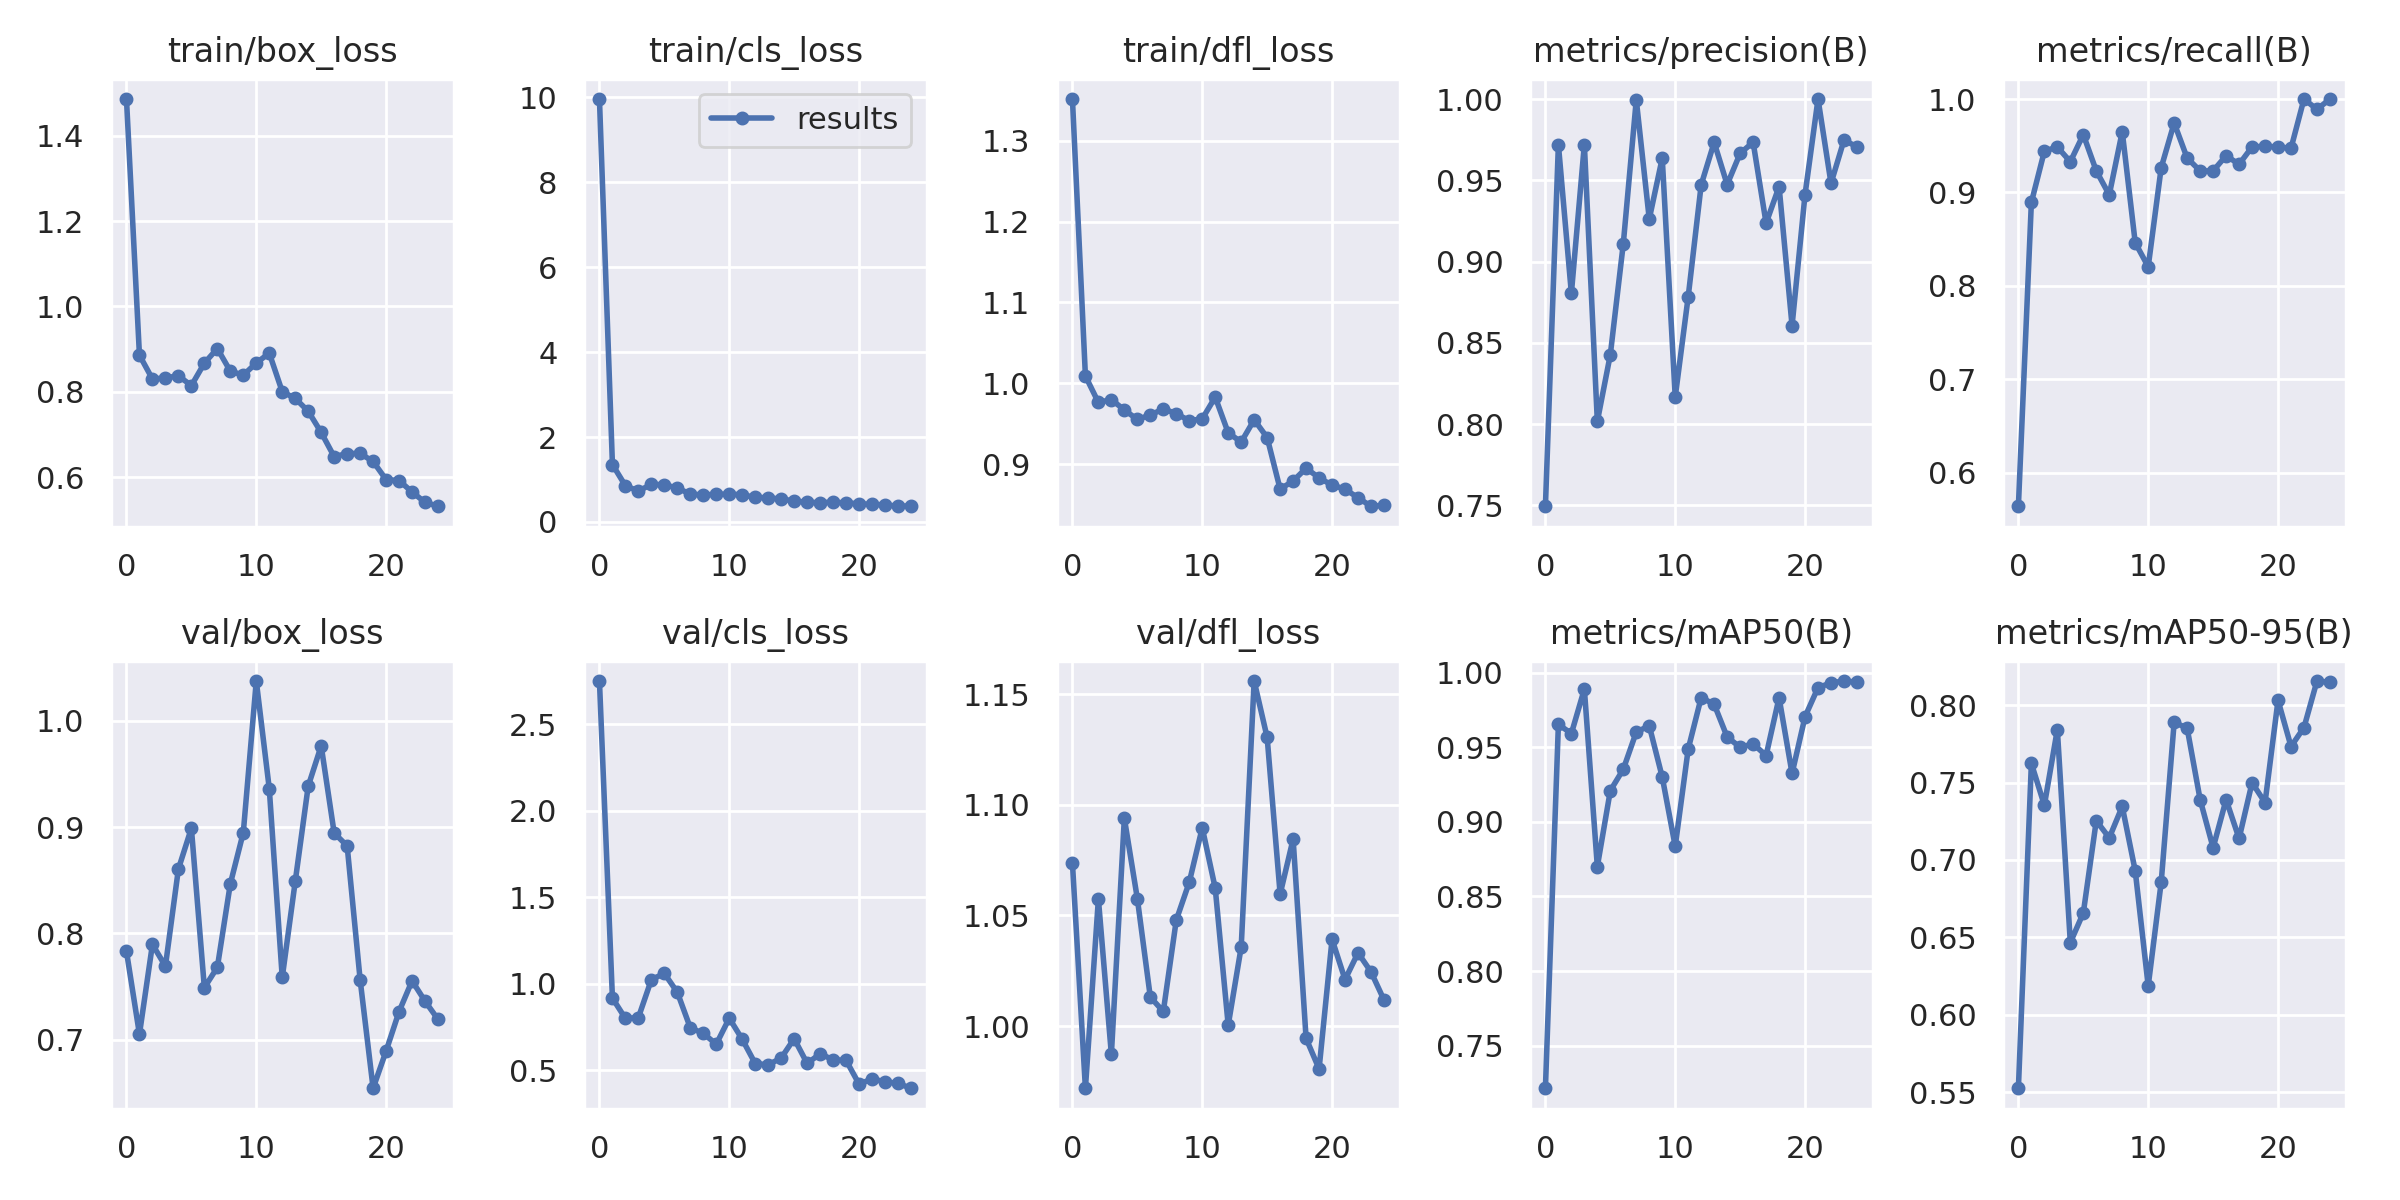
\includegraphics[width=0.8\linewidth]{results_small dataset.png}
    \caption{Results from \cite{carplate-xuk6s_dataset}}
    \label{fig:mesh1}
\end{figure}

The second dataset \cite{tablice-73he1_dataset} used contained 8683 images of which 6083 were for training, 1733 for validation and 867 for testing.The authors reported the following results with the yolov5 model, mAP: 84.7\%, Precision: 88.8\% and Recall: 80.8\%. In the figure [\ref{fig:mesh2}], is possible to see more details. A more detailed description of the meaning of these graphs will be give in the next section.

\begin{figure}[H]
    \centering
    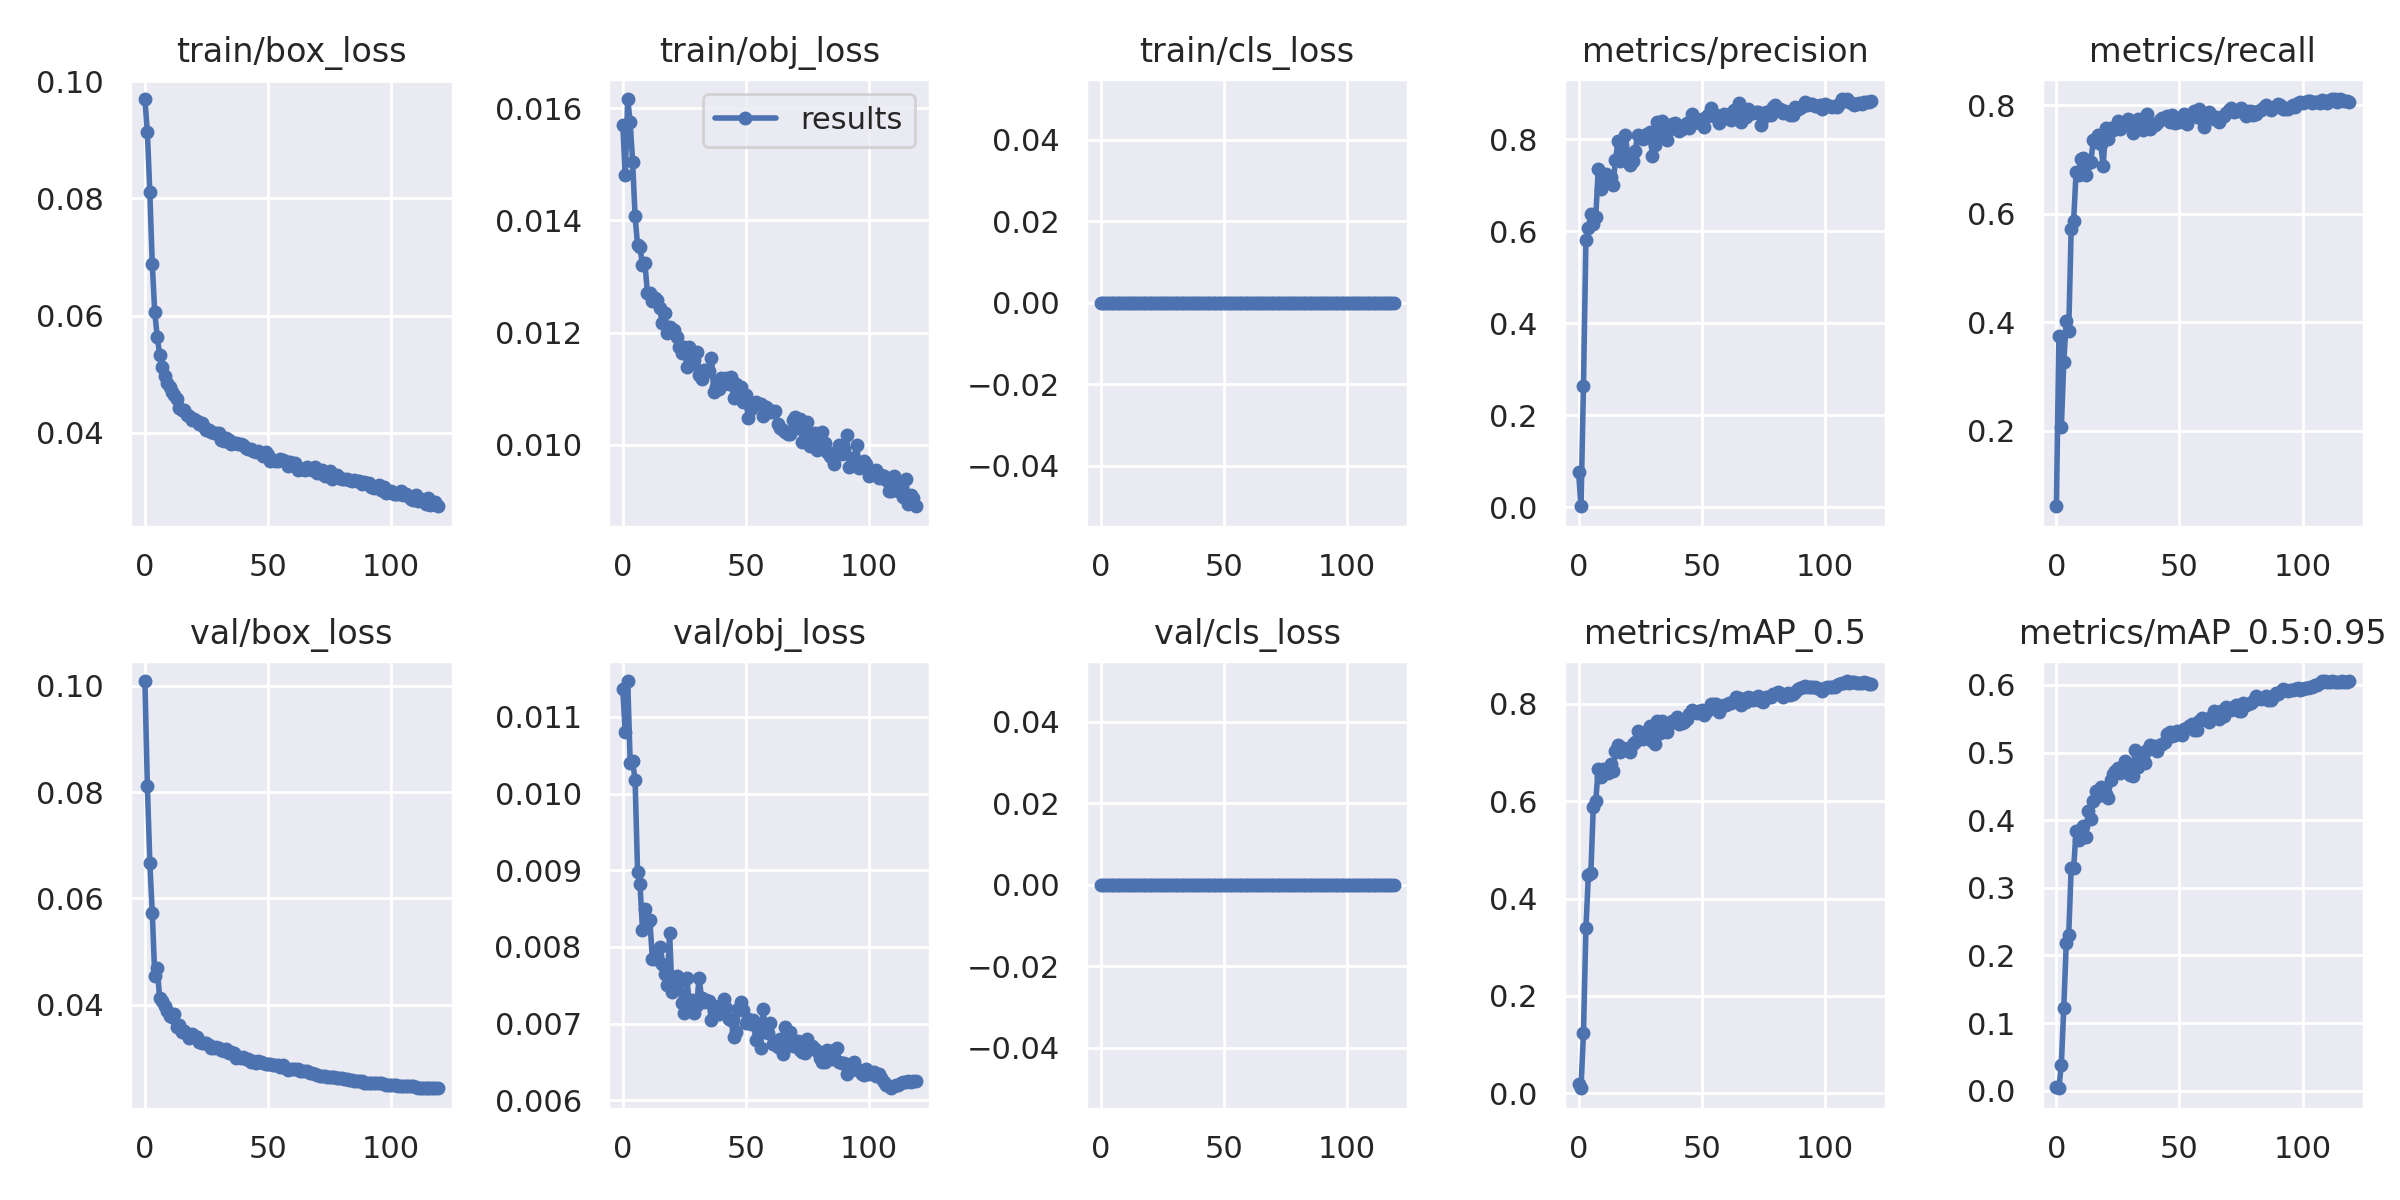
\includegraphics[width=0.8\linewidth]{results_big_dataset.png}
    \caption{Results from \cite{tablice-73he1_dataset}}
    \label{fig:mesh2}
\end{figure}


%%%%%%%%%%%%%%%%%%%%%%%%%%%%%%%%%%%%%%%%%%%%%%%%%%%%%%%%%%%%%%%%%%%%%%%%%%%%%%%%%%%%%%%%

\section{Training and results}
Training was performed using the yolov8n model, in a first step, using the dataset from about 300 images. Then the second dataset was used so as to analyze, also qualitatively the impact of the starting dataset on the achievable performance. Both tests were performed on 100 epochs. In the images [\ref{fig:mesh3}] and [\ref{fig:mesh4}] the results generated by the model can be observed.
\begin{figure}[H]
    \centering
    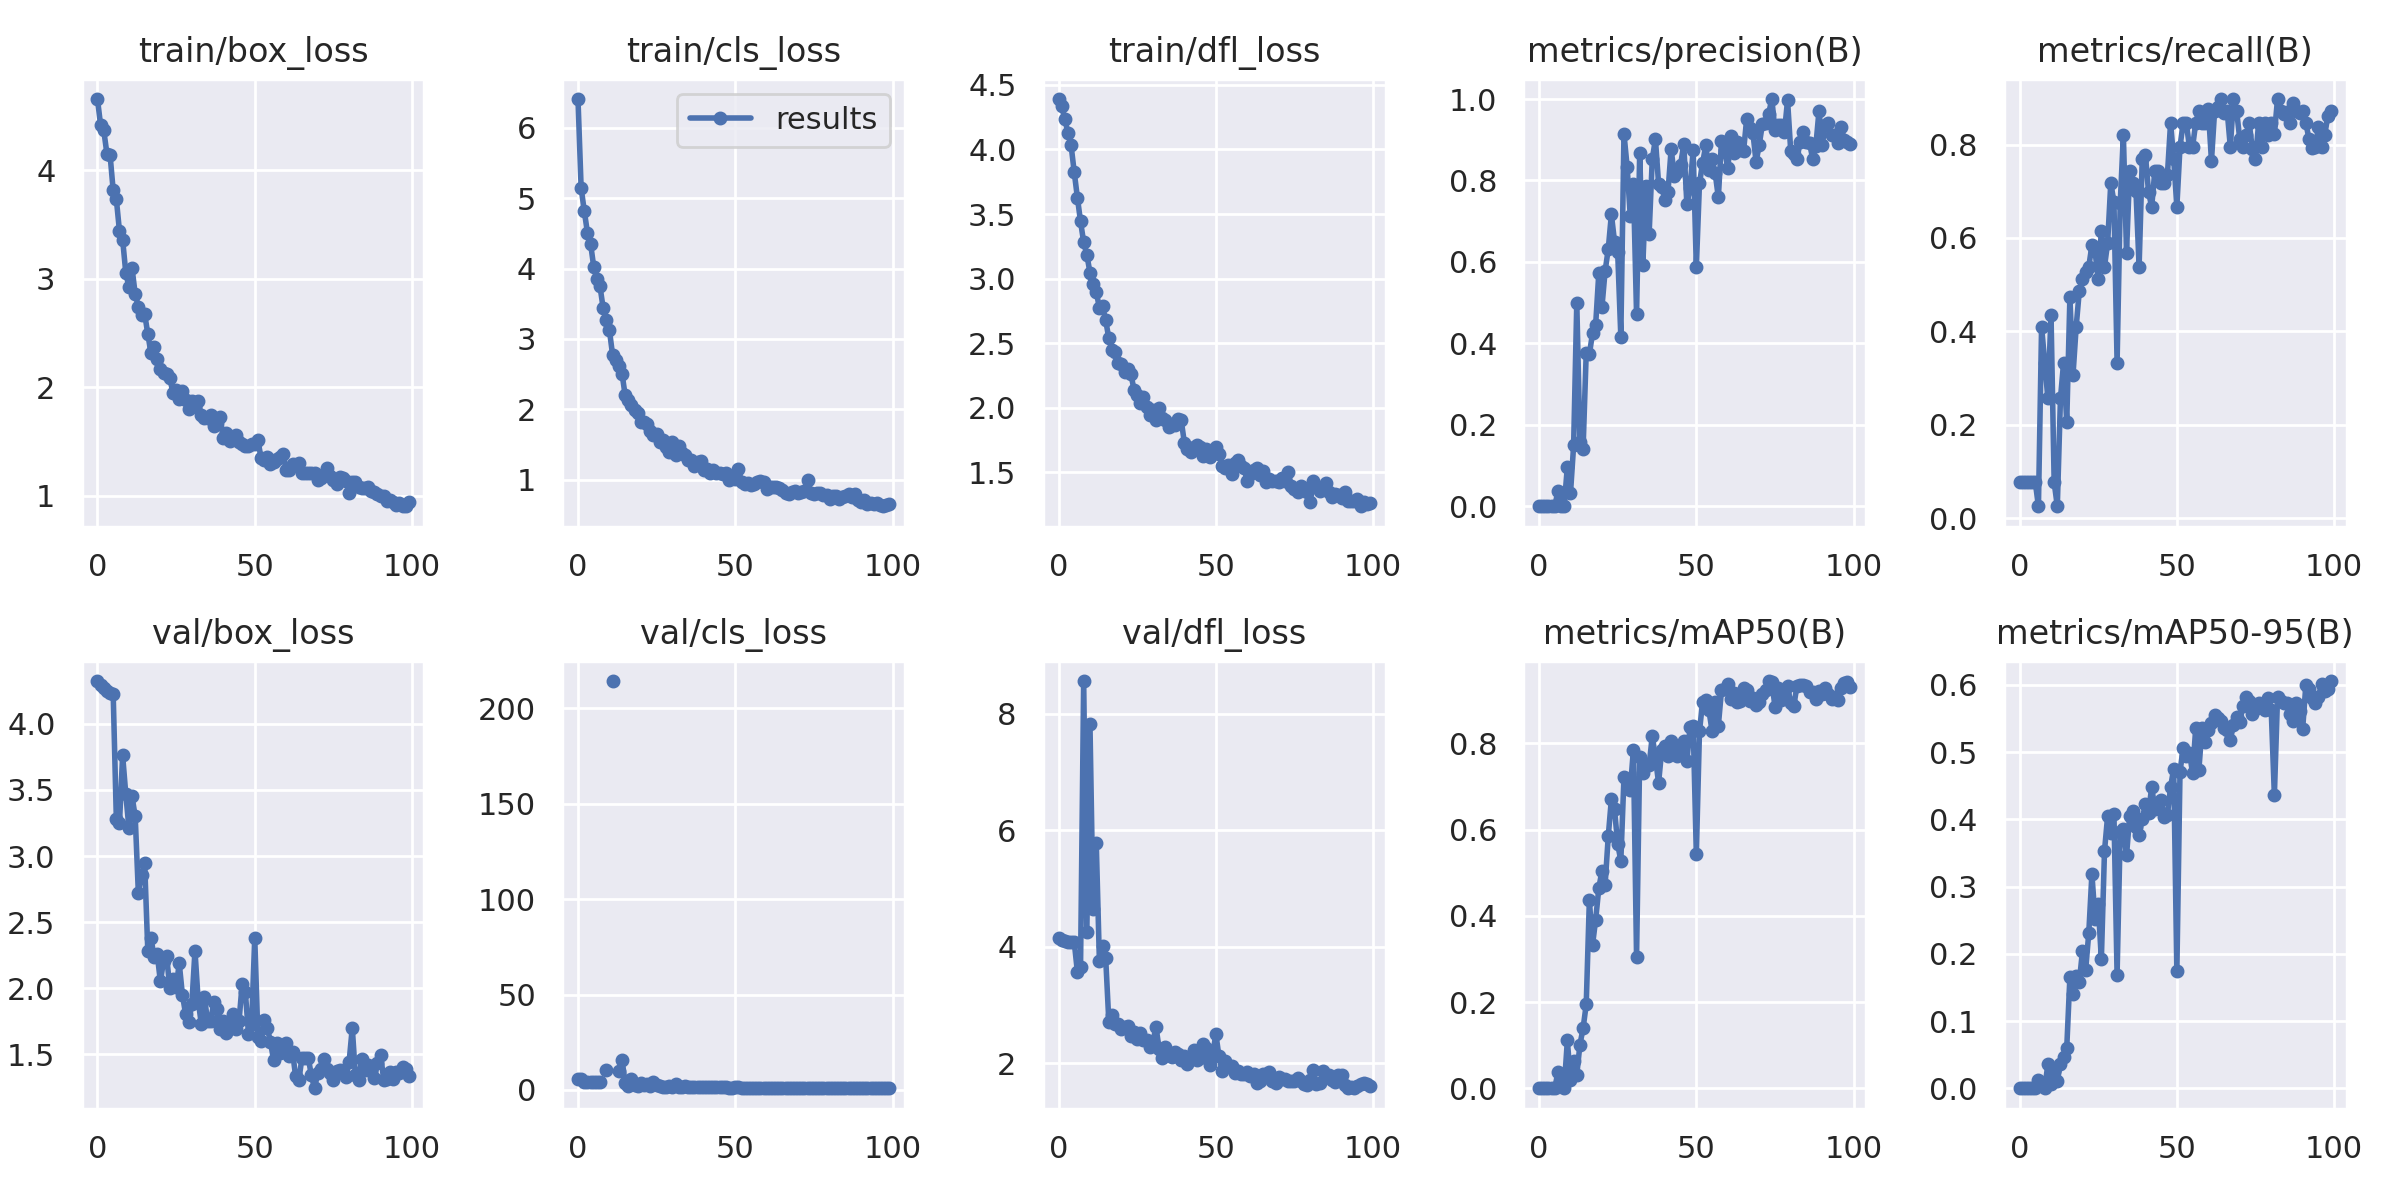
\includegraphics[width=0.8\linewidth]
    {results_training_small.png}
    \caption{Result after training with the small dataset \cite{carplate-xuk6s_dataset}}
    \label{fig:mesh3}
\end{figure}
\begin{figure}[H]
    \centering
    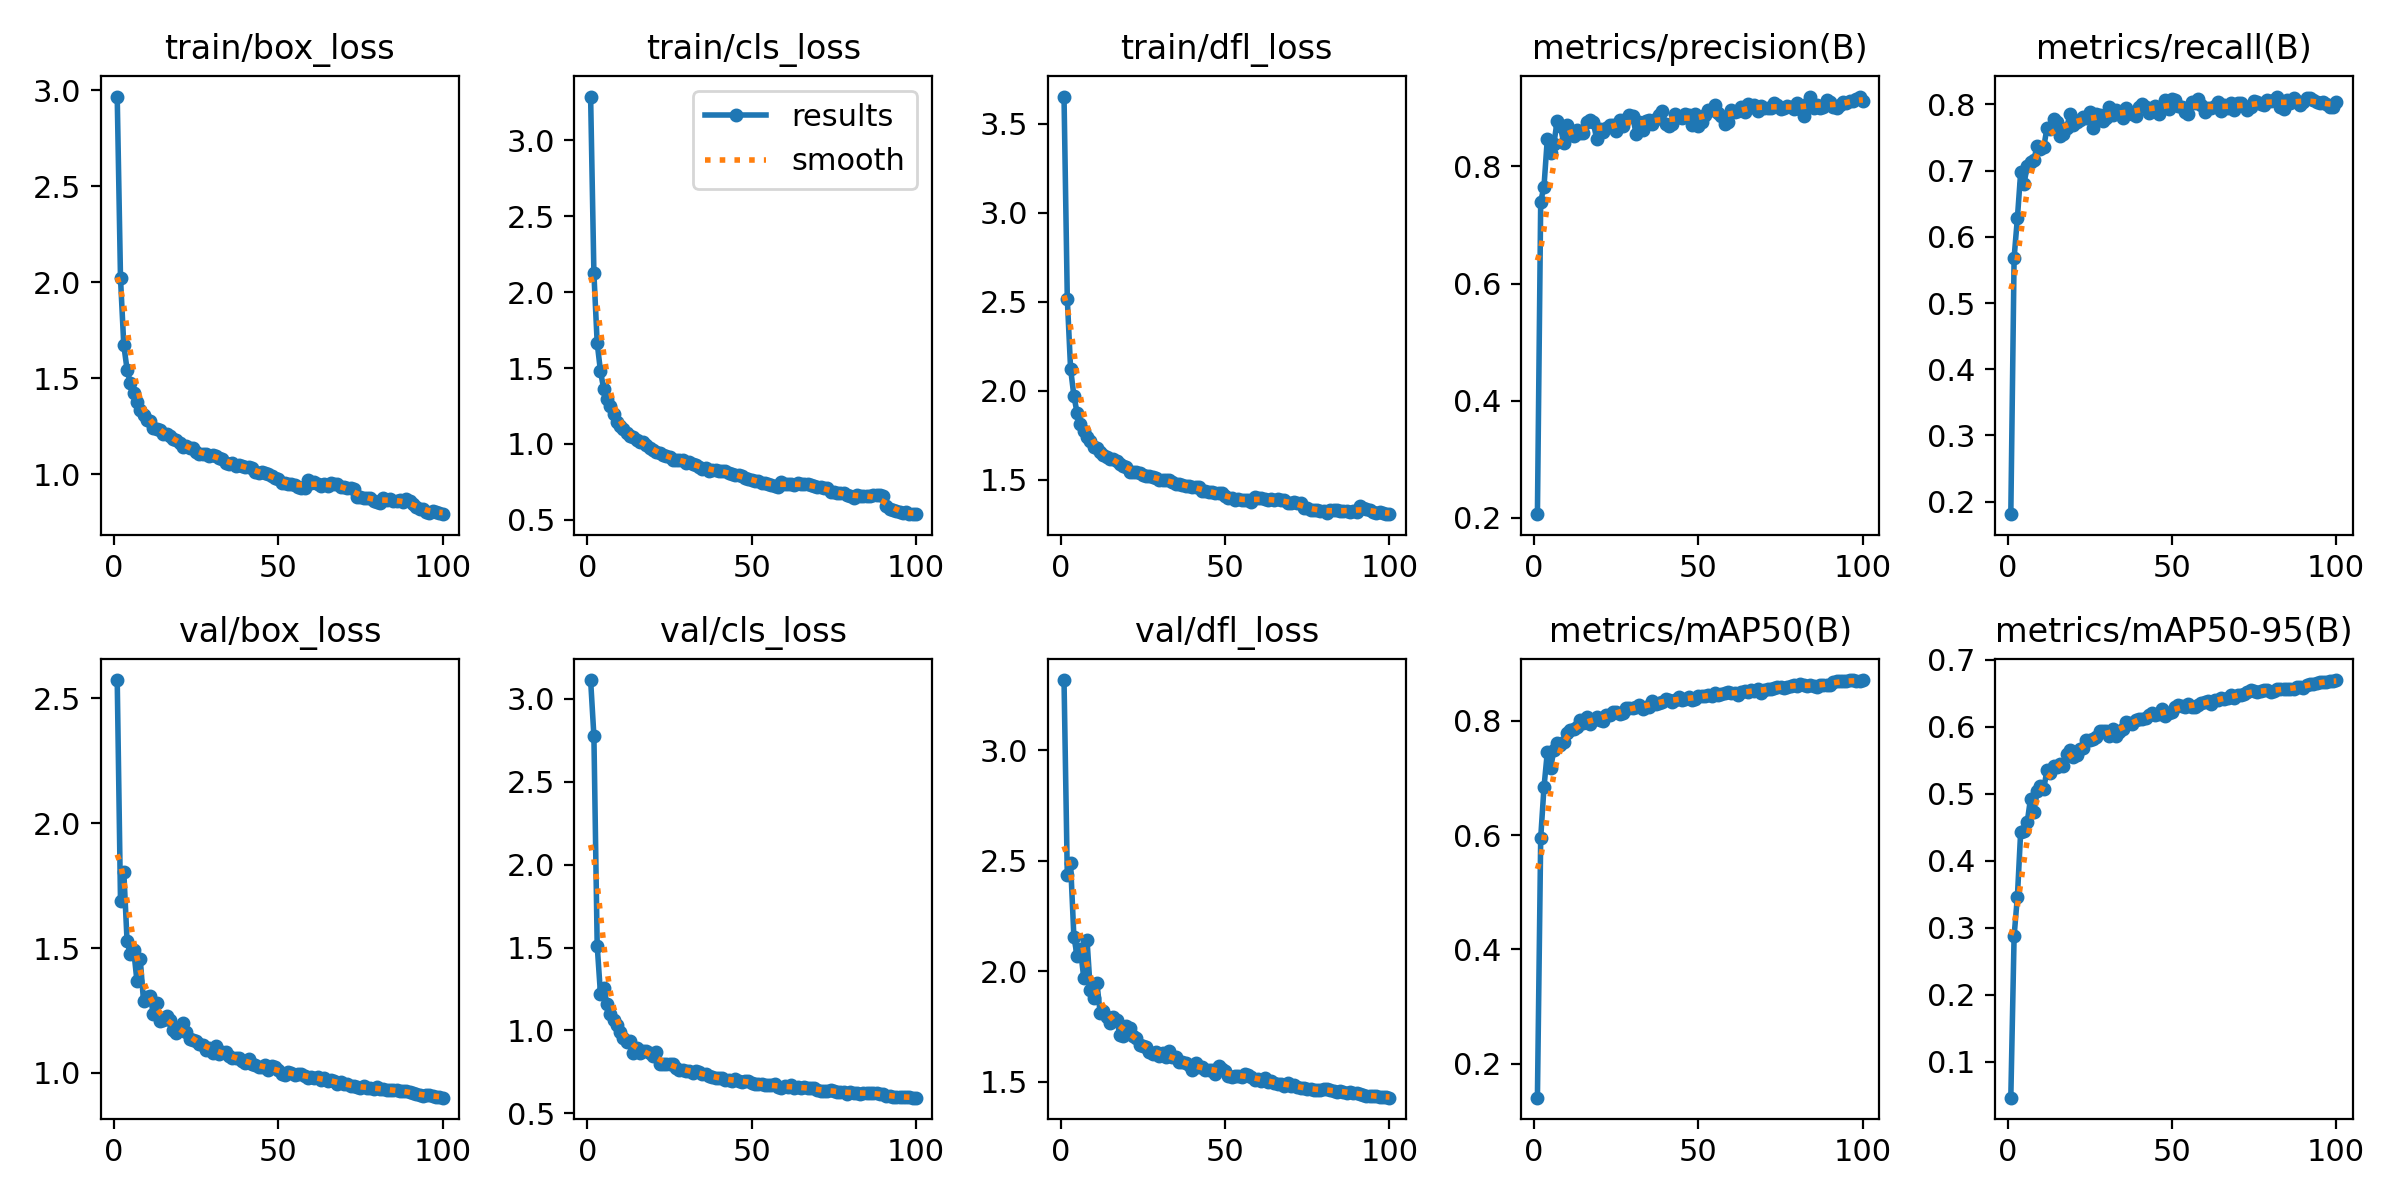
\includegraphics[width=0.8\linewidth]
    {results_training_big.png}
    \caption{Result after training with the big dataset \cite{tablice-73he1_dataset}}
    \label{fig:mesh4}
\end{figure}
Within these graphs, we can observe on the X-axis the number of epochs correspondent for each point on the Y-axis. The number of epochs represents "the number of times all training data passes through the model architecture" \cite{yolo2}.

The Y-axis can take on different meanings, in particular here we have five different metrics:
\begin{itemize}
    \item Box loss: this parameter represent a loss metric and in general, a lower value means better performance. It represents the accuracy with which the box containing the plate is defined compared to the box given as input;
    \item Class loss: It is another loss metric, but it refers to the capability of the model on classifying objects;
    \item mPA: this metric represents a summary of the previous two metrics by evaluating the average accuracy over all the data. This datum is usually referred to the Intersection over Union (IoU), defined as a value proportional to the area given by the intersection of the true bounded box and the predicted bounded box.Compared to this usually the mPA 50 and mPa 50:95 are given, where 50 and 95 represent the percentage of overlap between the bounded boxes;
    \item Precision: this parameter represents the accuracy of the model, defined simply as the ratio of the number of bounded boxes revealed to their actual number;
    \item Recall: this metric, unlike Precision,  relates the number of true bounded boxes to the total number of predicted bounded boxes among which there may be false positives.
\end{itemize}

These metrics, as can be seen in the figures, were evaluated for the images used during the training and for a different set (the validation set). The main differences can be observed in the loss metrics that did not reach values the same values. As can be seen from a comparison of the figures [\ref{fig:mesh1}] and [\ref{fig:mesh2}], with [\ref{fig:mesh3}] and [\ref{fig:mesh4}], respectively, the results obtained do not differ significantly except for the loss metrics. In particular, this may be due to the use by the authors of the two datasets of pre-trained models and larger models in general. Recall that the results obtained from this project are from the smaller Yolo V8 model. Also note the irregularity in the curves for the 300-image dataset due to the small number of data used.
In general however, it can be observed, as expected, that the model trained with more than 8000 images obtained better results in loss metrics than what was obtained using the small dataset, a difference that is less pronounced in terms of accuracy and mPA.

%%%%%%%%%%%%%%%%%%%%%%%%%%%%%%%%%%%%%%%%%%%%%%%%%%%%%%%%%%%%%%%%%%%%%%%%%%%%%%%%%%%%%%%%

\section{Conclusion and possible developments for the project}
In conclusion in this project training was performed with two different datasets of the Yolo V8 nano model. The model also generated data to evaluate the performance of the model and were compared with the results obtained by the authors of the two datasets. Next, a tracking test was performed although it is only mentioned in this report. An excerpt of the output video can be observed in figure [\ref{fig:mesh5}]. The demo video was taken from \cite{github2}.

\begin{figure}[H]
    \centering
    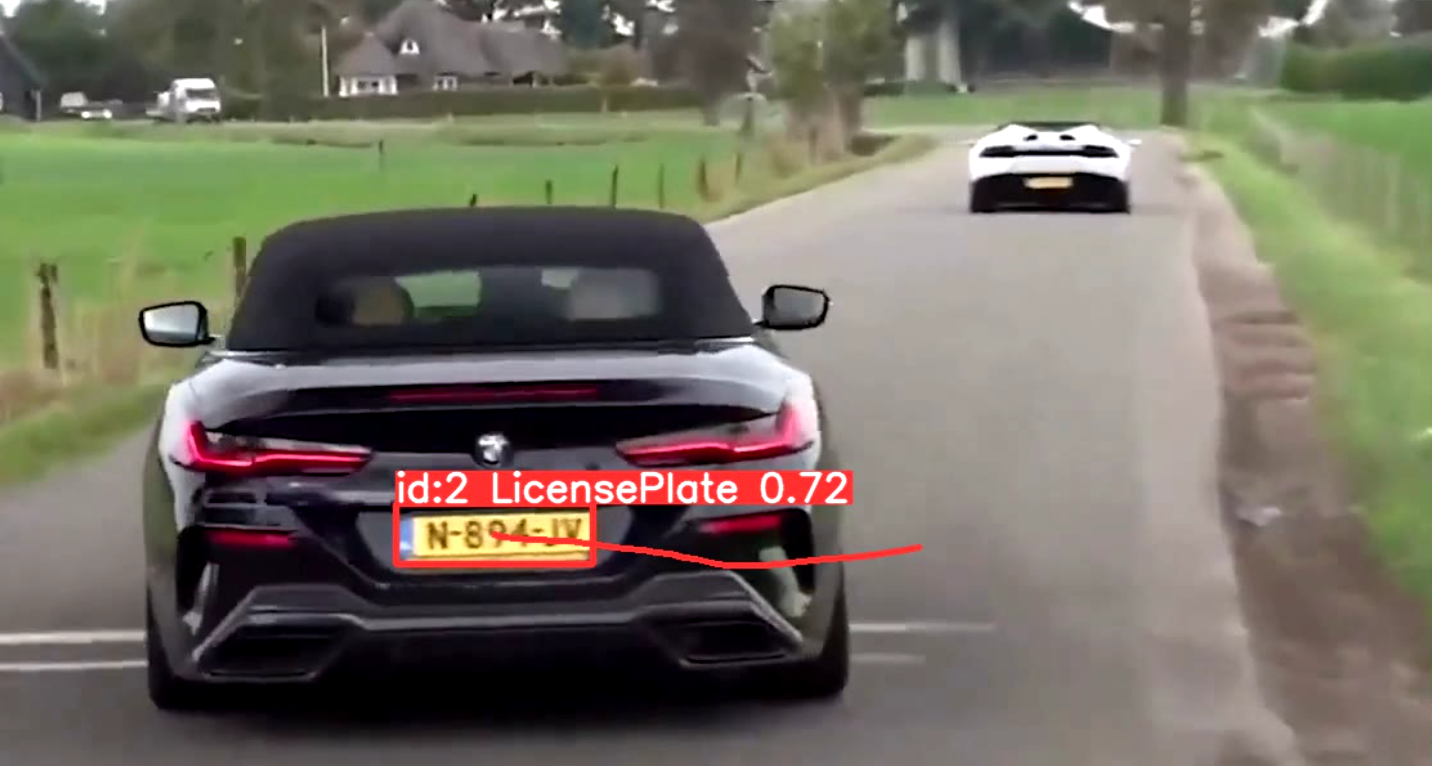
\includegraphics[width=0.5\linewidth]{tracking example.png}
    \caption{Result of the trained model used to perform tracking}
    \label{fig:mesh5}
\end{figure}
One possible development for this project that has not been pursued here is the ability to read license plates. Through Optical Character Recognition (OCR) it is indeed possible to implement a license plate reader that allows, once identified with Yolo, the text inside to be read and extracted. One such project can be observed in \cite{github1}.

%%%%%%%%%%%%%%%%%%%%%%%%%%%%%%%%%%%%%%%%%%%%%%%%%%%%%%%%%%%%%%%%%%%%%%%%%%%%%%%%%%%%%%%%

\clearpage

\bibliographystyle{ieeetr}
\begin{flushleft}
  \bibliography{main}
\end{flushleft}

%\appendix
%\newpage
%\section{}

\end{document}
